\begin{tcolorbox}
\chapter{2012 --- Sledi Vetra}

Sledi Vetra 2012 was a clear success. 2703 m of new cave passage was
found, the majority of which below -600 m, once again using Camp
\emph{X-Ray} at -550 m as a base. The main discoveries in
\emph{Vrtnarija} include: the \emph{Watership Down} series below
Daydreamers, adding 12 m of depth to the cave and taking it to -900 m;
about 1 km of horizontal development below \emph{Stuck in Paradise}
(-700 m); and the \emph{Apollo} extensions leading off a bolt climb in
the \emph{Queen's Bedchamber}. The \emph{Apollo} extensions also ended
up connecting to \emph{Waterloo} in System Migovec, giving us the long
sought after connection and tying in \textasciitilde 15 years of
exploration by ICCC on Migovec. System Migovec is now 25592 m long, 973
m deep and has the distinction of being the longest cave in Slovenia.

\end{tcolorbox}
\backgroundsetup{
    scale=1,
    color=black,
    opacity=1,
    angle=0,
    contents={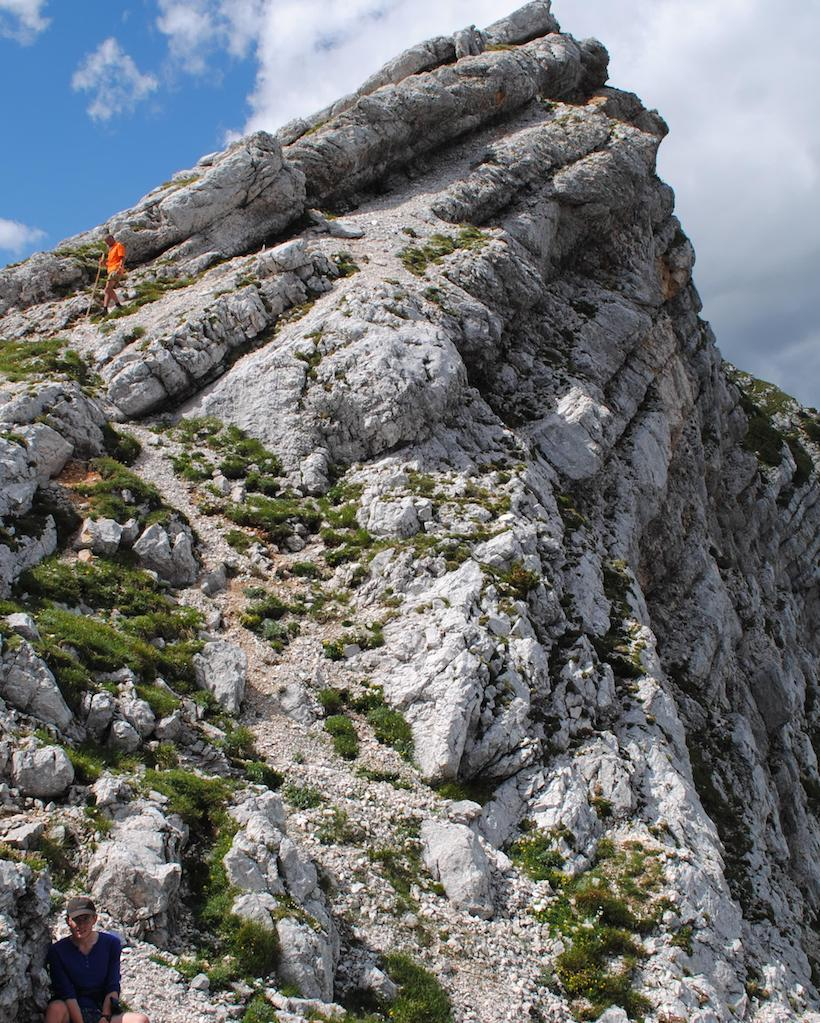
\includegraphics[height=\paperheight]{2007/intro/kuk-2013.jpg}}
}
\BgThispage









